\documentclass[aspectratio=169]{beamer}
% TODO cambiar a la de dalt
%\documentclass[aspectratio=169,handout]{beamer}
\usepackage{pgfpages}

%
% ============ APARTATS ============
% i) Definició del models SUM I MAX.
% ii) Computar la Best response és NP-hard en el dos models (SUM I MAX) 
%     (Theorem 1 i doneu tots els details que pugueu tan per MAX com per SUM)
%

% ============== TODO ===============
% - Network Creation Games:
%    + explicar PoS i PoA 
% - Model SUM: 
%    + diameter, etc
% - Model MAX:
%    + diameter, etc
% - k-MEDIAN
%    + explicar per sobre com sabem que es NP-hard
% - k-CENTER
%    + explicar per sobre com sabem que es NP-hard

%\setbeameroption{show only notes}
\setbeameroption{show notes on second screen}

\usepackage[catalan]{babel}
\usepackage[utf8]{inputenc}
\usepackage[T1]{fontenc}

\usepackage[style=english]{csquotes}

\usepackage[
backend=biber,
%style=apa,
%sorting=ynt
]{biblatex}
\addbibresource{biblio.bib}

\usetheme{Madrid}
\useinnertheme{rectangles}
\usefonttheme{professionalfonts}
\usecolortheme{crane}
\setbeamertemplate{blocks}[default]
\setbeamersize{text margin left=10mm,text margin right=10mm} 

\usepackage{times} 
\usepackage{booktabs}
\usepackage[scale=2]{ccicons}
\usepackage{xspace}
\usepackage{graphicx}
%\usepackage{enumitem}

\usepackage{amsmath}
\usepackage{tikz}

\DeclareMathOperator{\dist}{dist}
\DeclareMathOperator{\SUM}{SUM}
\DeclareMathOperator{\MAX}{MAX}

\newcommand{\kcenter}{\texorpdfstring{$k$}{k}-\textsc{center}\xspace}
\newcommand{\kmedian}{\texorpdfstring{$k$}{k}-\textsc{median}\xspace}

\setbeamercovered{transparent}

\title[Bounded Budget Network Creation Game]{Bounded Budget Network Creation Game}
\subtitle{}
\author{Grup 1}
\institute{UPC - AA}
\date{10 de juny de 2020}

\begin{document}

\begin{frame}
  \titlepage
  \note{hello}
  \note[item]{test}
\end{frame}

\begin{frame}{Index}
  \tableofcontents
\end{frame}

\section{Introducció}

\begin{frame}{Introducció}
    \setlength{\leftmargini}{10em}
    \begin{itemize}
        \itemsep=1em
        \item[\textbf{Article:}] Bounded Budget Network Creation Game
        \item[\textbf{Autors:}] Sayan Ehsani, Saber Shokat Fadaee, Mohammadamin Fazli, Abbas Mehrabian, Sina Sadeghian Sadeghabad, Mohammadali Safari and Morteza Saghafian
        \item[\textbf{Publicació:}] ACM Transaction on Algorithms, Vol. 11, No. 4, Article 34
        \item[\textbf{Data de publicació:}] Abril 2015
        \item[\textbf{DOI:}] 10.1145/2701615
    \end{itemize}
\end{frame}

\subsection{Network Creation Games}
\setbeamercovered{transparent}
\begin{frame}{Network Creation Games}
    %Un Network Creation Game és un joc que modela la creació d'una xarxa a través d'un graf.
    
    \onslide<1->{Un \emph{Network creation game} es centra en \textbf{modelar xarxes} de la vida real des del punt de vista de la \textbf{teoria de jocs}.}
    
    \vspace{1em}
    
    % nose
    
    % Selfish Network Creation focuses on modeling real world networks from a game-theoretic pointof view. 
    % One of the classic models by Fabrikant et al. [PODC’03] is the network creation game,where agents correspond 
    % to nodes in a network which buy incident edges for the price ofαperedge to minimize their total distance to all other nodes

\note{
 Hi ha moltes variants de jocs. La que expliquem aquí es la mes típica (la d classe).
 La que s estudia al paper es un altre que no te $\alpha$
}
    
    \onslide<2->{\textbf{Cada node $u$ representa un jugador} i \textbf{cada jugador té una estratègia $S_u$}, representada per un conjunt d'arestes que el jugador
    crea, on cada aresta té cost de creació $\alpha$.}
    
    \vspace{1em}
    
    \onslide<3->{El vector d'estratègia $S = (S_1,...,S_n)$ conté l'estratègia de cada jugador i $G(S)$ és el graf no-dirigit resultant d'aplicar les estratègies.}
    
    \vspace{1em}
    
    \onslide<4->{\textbf{Objectiu} de cada node:
    \begin{itemize}
        \item Minimitzar la creació d'arestes
        \item Minimitzar la distància als altres nodes
    \end{itemize}}
\end{frame}

\begin{frame}{Network Creation Games}
    Cada node vol minimitzar la seva funció de cost, que definim com:
    \begin{equation*}
        C(u) = \alpha n_u + \sum_{v \in V(G)}\dist(u,v)
    \end{equation*}
    on $n_u = |S_u|$ i $G$ és el graf que representa la xarxa.
    
    \vspace{1em}
    
    Definim el \textbf{cost social} com la suma dels costos de tots els nodes:
    \begin{equation*}
        SC(S) = \alpha |E| + \sum_{u,v \in V(G)} \dist(u,v)
    \end{equation*}
\end{frame}

\subsection{Bounded Budget Network Creation Game}
\begin{frame}{Bounded Budget Network Creation Game}
Definicions:
\begin{itemize}
    \item<1-> Donat un graf dirigit $G$, denotem el seu conjunt de vèrtexs com $V(G)$.
    \item<2-> $U(G)$ es un graf no-dirigit obtingut ignorant les direccions en $G$.
    \item<3-> Si $\vec{uv}, \vec{vu} \in G$ llavors $uv \in U(G)$ te multiplicitat 2 i
        anomenem la parella $\{u, v\}$ \emph{brace}.
    \item<4-> $\dist(u, v)$ denota la distancia entre $u$ i $v$ a $U(G)$.
    \item<5-> Si $u$ i $v$ estan en components connexos diferents de $U(G)$ llavors
        $\dist(u, v) = C_{inf} = n^2$.
    \item<6-> No tenim $\alpha$, es a dir, les arestes no tenen cost.
        
    \note{El motiu del valor de $C_{inf} = n^2$ s'explica mes endavant}
    
\end{itemize}
\end{frame} 

\begin{frame}{Bounded Budget Network Creation Game}
    Denotem un \emph{Bounded budget network creation game} com:
    $$ (b_1, b_2, \dots , b_n)\text{-BG} $$
    On $b_1,b_2, \dots , b_n$ son enters no negatius que representen el \emph{budget} de cada jugador ($n$ es el nombre de jugadors).
    
    \vspace{1em}
    
    Cada jugador $i$ te assignada una estratègia $S_i \subseteq \{1, 2, \dots , n\} \backslash \{i\}$ amb
    $|S_i| = b_i$
    
    \vspace{1em}
    
    Podem construir un graf $G$ a partir del conjunt de totes les estratègies afegint un vèrtex $\vec{u_iv_j}$
    a $G$ si i nomes si $j \in S_i$. Anomenen a aquests grafs \emph{realitzadors} de
    $ (b_1, b_2, \dots , b_n)\text{-BG} $.
    
    \vspace{1em}
    
    Direm que un vèrtex esta en la millor resposta (\emph{best response}) si no pot disminuir el seu
    cost mantenint fixes les estratègies de la resta de vèrtexs.
\end{frame}

\subsection{Resultats}
\begin{frame}{Resultats}
% yes?
% idk , nice XD
% no se si aqui o en la explicacion del paper.
% ya, es mi otra opcion jajaja 
% en el paper hablan de los results de todo, nosotros solo comentamos de nuestra parte o de todo?
% tal como lo decia merca es comentar todo. en plan como explicar lo que dice en el abstract basicamente.
% por eso que igual mejor al principio, pero ni idea. Tambien depende de k digas o como lo digas.
% idk
% ok
% okay pue primero hacemos la diapo y pensamos que decir y luego vemos si delante o detras (btw creo que mejor delante)+1
% lo pongo delante y luego ya si eso lo movemos

% mmmhhh qiuzas al menos se tendria que poner despues de nombrar las dos versiones

% exacto o al final, pq son las conclusiones del paper 
% ya, pero no son las conclusiones de lo nuestro, nose

Es demostra que:
\begin{itemize}
    % Primer de tot es demostra que
    \item Per tota seqüencia no negativa $ (b_1, b_2, \dots , b_n)$ en el joc $ (b_1, b_2, \dots , b_n)\text{-BG} $ hi ha un equilibri de Nash pur i el preu d'estabilitat és $\Theta(1)$ en les dues versions.
    
    \vspace{1em}
    
    \item En els casos on la suma dels pressuposts és igual a $n-1$ el \emph{PoA}
    és~$\Theta(n)$ i~$\Theta(\log n)$ en~$\MAX$ i~$\SUM$ respectivament.
    
    \vspace{1em}
    
    \item El \emph{PoA} quan el pressupost de tots els jugadors és igual a $1$ és $\Theta(1)$ en les dues versions.
    
    % 1em es la altura de una M mayusulca, mas facil de ver k los mm imo.
    % Xd
    % tambien hay ex k es la x minuscula.
    % interesting jajaj todos los dias se aprende algo nuevo con \LaTeixB

    \vspace{1em} % mejor usar em en vez de mm.
    % yo lo he copiado de las diaps de arriba pues yo siempre uso em, alguien lo ha cambiado XD
    % k en verdad da igual, pero em depende del tamano de la letra, no de la mida de la pantalla.
    % como no cambiaremos el tamano de las diapos suda.
    % te habias dejado 2 "3mm" nice
    
    \item A mesura que s'incrementa el pressupost dels jugadors el diàmetre del graf \textbf{no} disminueix. Per la versió de $\MAX$ hi han instàncies amb tots el pressuposts positius on el PoA és $\Omega(\sqrt{\log n})$.
    
    \vspace{1em}
    
    \item 
    
    % y si no ponemos este texto inicial? en plan no hace falta escribirlo todo, uno de nosotros ya lo explicara 
    % lo podemos poner en la note y que quien diga esta parte lo comente
    % exacto
    \note{Al paper s'estudien diverses propietats dels \emph{equilibrium graphs}. En particular s'analitza el diàmetre dels grafs en alguns casos especials. Aquest anàlisi resulta en uns límits del preu de l'anarquia (PoA) pels diferents casos.}
    
\end{itemize}

\end{frame}


\section{Definició dels models}

\begin{frame}{Definició dels models}
    En el paper\cite{ehsani_bounded_2015} es consideren 2 models de \emph{bounded budget network creation games}:
    
    \vspace{1.5em}
    
    \begin{itemize}
    \item $\SUM$
    \item $\MAX$
    \end{itemize}
    
    \vspace{3em}
    
    Els models difereixen en la definició de la funció de cost.
\end{frame}

\subsection{\texorpdfstring{$\SUM$}{SUM}}
\begin{frame}{Model $\SUM$}

Definim la funció de cost del model $\SUM$ com:

\begin{equation}
    c_{\SUM}(u) = \sum_{v \in V(G)} \dist(u, v)
\end{equation}

\note{
Com que $C_{inf} = n^2$ es garanteix que si un canvi d estratègia en u disminueix
el nombre de components connexos $c_{\MAX}$ es redueix.

Per tant s incentiva la reducció de components connexos al igual que a $\SUM$.
}

\end{frame}

\subsection{\texorpdfstring{$\MAX$}{MAX}}
\begin{frame}{Model $\MAX$}

Definim la funció de cost del model $\MAX$ com:

\begin{equation}
    c_{\MAX}(u) = \max \{ \dist(u, v) : v \in V(G) \} + (\kappa - 1)n^2
\end{equation}

On $\kappa$ es el nombre de components connexos de $U(G)$.

\vspace{2em}

El primer terme $\max \{ \dist(u, v) : v \in V(G) \}$ es l'excentricitat de $u$.

El terme $(\kappa - 1)n^2$ s'afegeix per incentivar decréixer el nombre de components connexos.

\end{frame}

\section{Computar best response \'{e}s NP-hard en ambdós models}
\subsection{Theorem 2.1}
\begin{frame}{Teorema}

    Al paper s'enuncia i demostra el següent teorema:
    
    \begin{theorem}
    The problem of finding a player's best response in both $\MAX$ and $\SUM$ versions of the bounded
    budget network creation games is NP-hard.
    \end{theorem}
    
    \vspace{2em}
    
    La demostració es basa en una reducció de \kcenter a $\MAX$ i de \kmedian a $\SUM$.
    On \kcenter i \kmedian són 
    NP-hard~\cite{hsu_easy_1979,lin_e-approximations_1992,megiddo_complexity_1984}.
    
\end{frame}

\begin{frame}{Papers citats}
\begin{columns}

\begin{column}{0.5\textwidth}
\begin{figure}
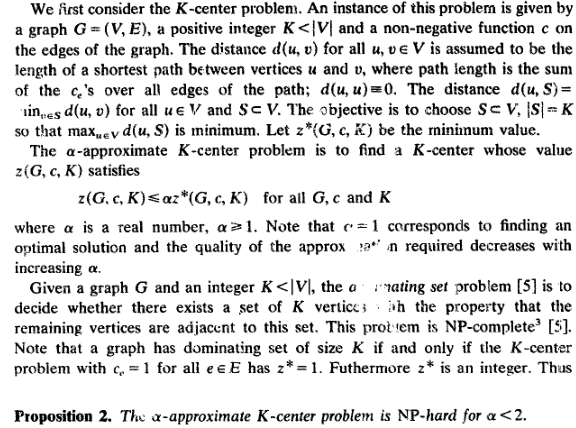
\includegraphics[width=\textwidth]{k-center_dominating_set}
\caption{Wen-Lian Hsu i George L. Nemhauser. (1979) \cite{hsu_easy_1979} }
\end{figure}

\note[item] {
    Al paper de Wen-Lian \textbf{Hsu} i George L. \textbf{Nemhauser} es demostra que \kcenter es NP-hard fent una reduccio
    de \emph{dominating set}.
    \item Al paper de \textbf{Lin i Vitter} al que fa referencia el nostre paper original per referirse a la definicio
    de \kmedian, citen al paper de \textbf{Meggido i Supowit} en el que es demostren tant \kmedian com \kcenter
    fent reduccions a 3-SAT.
}
\end{column}

\begin{column}{0.5\textwidth}
\begin{figure}
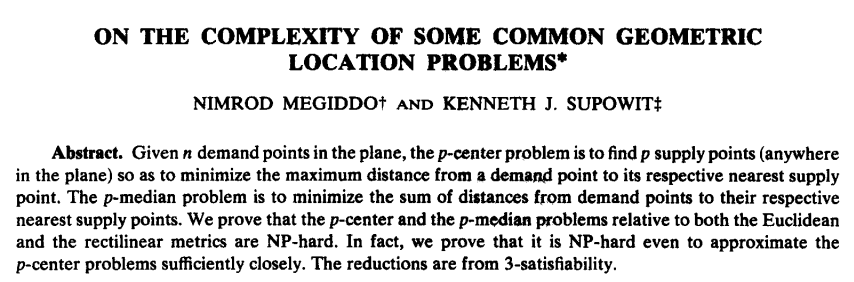
\includegraphics[width=\textwidth]{abstract_megiddo}
\caption{Nimrod Megiddo i Kenneth Supowit. (1984) \cite{megiddo_complexity_1984} }
\end{figure}
\end{column}

\end{columns}
\end{frame}

\subsection{\kcenter}
\begin{frame}{\kcenter}

\begin{problem}[\kcenter]
Donat un graf no-dirigit $H$ i un enter positiu $k$ es vol trobar un subconjunt $S$ de $k$
vèrtexs que minimitzi la distancia màxima de un vèrtex a $S$:

\begin{equation}
\min_{S \subseteq V(H):|S|=k} \left( \max_{v \in V(H)} \dist(v, S) \right)
\end{equation}
\end{problem}

\begin{equation}
    \dist(v, S) = \min \{ \dist(v, u) : u \in S \}
\end{equation}

\end{frame}

\subsection{Reducció de \kcenter a \texorpdfstring{$\MAX$}{MAX}}
\begin{frame}{Reducció de \kcenter a $\MAX$}
    Donat un graf no dirigit $H$ de $n$ vèrtexs i un enter positiu $k$ volem trobar una solució òptima a
    \kcenter.
    
    \vspace{2em}
    
    Considerem ara un graf $G$ tal que $U(G) = H$ i un joc $ (b_1, b_2, \dots , b_n, b_{n+1})\text{-BG} $ on
    $b_i$ es el grau de sortida del vèrtex $i$ de $G$ i $b_{n+1} = k$.
    
    \vspace{2em}
    
    La millor resposta (\emph{best response}) del jugador $n+1$ amb les estratègies de la resta marcades
    per $G$ es una solució òptima de \kcenter.
    
    \note{
        %TODO: explicar en detall aixo
        
        La distancia de qualsevol vèrtex a $n+1$ serà sempre 1 + la distancia a la solució de \kcenter (conjunt $S$)
    }
\end{frame}

%\begin{frame}
%\begin{tikzpicture}[shorten >=1pt,->]
%  \tikzstyle{vertex}=[circle,fill=black!25,minimum size=12pt,inner sep=2pt]
%  \node[vertex] (G_1) at (-1,-1) {1};
%  \node[vertex] (G_2) at (0,0)   {2};
%  \node[vertex] (G_3) at (1,-1)  {3};
%  \draw (G_1) -- (G_2) -- (G_3) -- cycle;
%\end{tikzpicture}
%\end{frame}

%\subsection{\kcenter NP-hard}
%\begin{frame}{\kcenter NP-hard}
%\cite{hsu_easy_1979}
%\end{frame}

\subsection{\kmedian}
\begin{frame}{\kmedian}

\begin{problem}[\kmedian]
Donat un graf no dirigit $H$ i un enter positiu $k$ es vol trobar un conjunt $S \subseteq V(H)$ de $k$ vèrtexs
tal que es minimitzi la suma de les distancies de cada vèrtex en $V(H)$ a el vèrtex mes proper
de $S$.

\begin{equation}
\min_{S \subseteq V(H):|S|=k} \left(
    \sum _{v \in V(G)} \dist(v, m_S(v))
\right)
\end{equation}

On $m_S(v)$ es el vèrtex de $S$ mes proper a $v$.
% quizas aqui podemos poner algo en plan m_S(v) = min_{u \in S} dist(u,v)

%Es pot formular el problema en termes de programació lineal de minimització:
%
%\begin{columns}[T]
%
%\begin{column}{0.49\textwidth}
%\begin{equation}
%    \sum_{i \in V} \sum_{j \in V} \dist(i, j)*x_{ij}
%\end{equation}
%\begin{align*}
%    x_{ij} &\leq y_j, &i,j \in V \\
%    x_{ij}, y_j &\in \{0, 1\}, &i,j \in V \\
%\end{align*}
%\end{column}
%
%\begin{column}{0.49\textwidth}
%\begin{align*}
%    \sum_{j \in V} x_{ij} &= 1, & i \in V \\
%    \sum_{j \in V} y_j &\leq k, \\
%\end{align*}
%\end{column}
%
%\end{columns}

\end{problem}

\end{frame}

\subsection{Reducció de \kmedian a \texorpdfstring{$\SUM$}{SUM}}
\begin{frame}{Reducció de \kmedian a $\SUM$}

Apliquem el mateix principi que en el cas de \kcenter i $\MAX$:

    \vspace{2em}

    Donat un graf no dirigit $H$ de $n$ vèrtexs i un enter positiu $k$ volem trobar una solució òptima a
    \kmedian.
    
    \vspace{2em}
    
    Considerem ara un graf $G$ tal que $U(G) = H$ i un joc $ (b_1, b_2, \dots , b_n, b_{n+1})\text{-BG} $ on
    $b_i$ es el grau de sortida del vèrtex $i$ de $G$ i $b_{n+1} = k$.
    
    \vspace{2em}
    
    La millor resposta (\emph{best response}) del jugador $n+1$ amb les estratègies de la resta marcades
    per $G$ es una solució òptima de \kmedian.
    
    \note{
        %TODO: explicar en detall aixo
        
        La distancia de qualsevol vèrtex a $n+1$ serà sempre 1 + la distancia a la solució de \kmedian (conjunt $S$)
        
        La suma es nomes dels elements mes propers, per tant es manté la condició de $\dist$ a $m_S(v)$
    }

\end{frame}


\begin{frame}{Bibliografia}
\printbibliography
\end{frame}

\begin{frame}
\end{frame}

\end{document}

